%\newpage
\chapter{Beschreibung der MOSFET-Messungen}
\label{sec:MOSmeasurements}

\begin{figure}[H]
  \begin{subfigure}[b]{.5\textwidth}
    \centering
    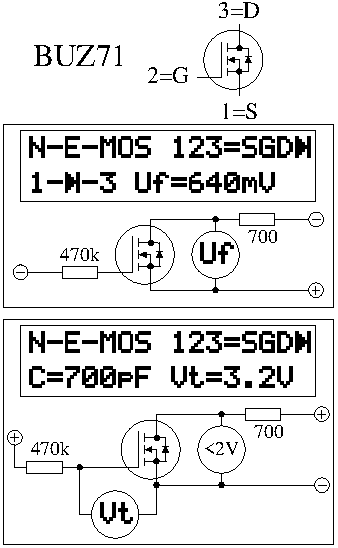
\includegraphics[width=1.\textwidth]{../FIG/MOS_BUZ71.pdf}
    \caption{N-E-MOSFET}
    \label{fig:MOS-N-E}
  \end{subfigure}
  ~
  \begin{subfigure}[b]{.5\textwidth}
    \centering
    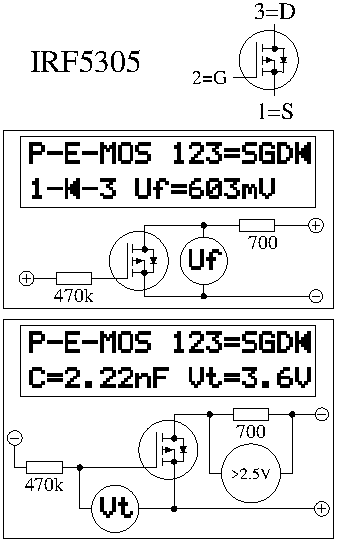
\includegraphics[width=1.\textwidth]{../FIG/MOS_IRF5305.pdf}
    \caption{P-E-MOSFET}
    \label{fig:MOS-P-E}
  \end{subfigure}
  \caption{Anreicherungs-MOSFETs}
\end{figure}



\begin{figure}[H]
\centering
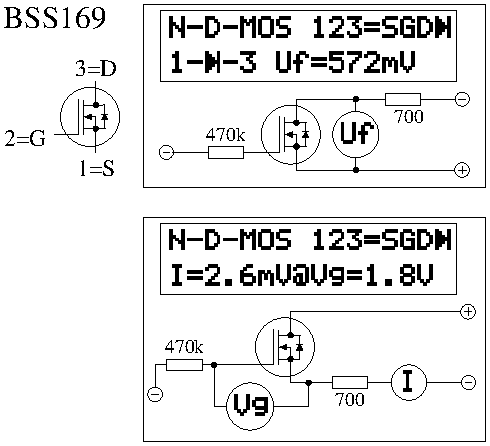
\includegraphics[]{../FIG/MOS_BSS169.pdf}
\caption{N-D-MOSFET}
\label{fig:MOS-N-D}
\end{figure}

\begin{figure}[H]
  \begin{subfigure}[b]{.5\textwidth}
    \centering
    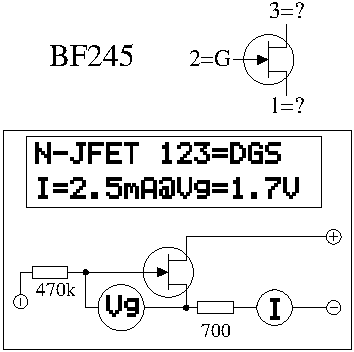
\includegraphics[width=1.\textwidth]{../FIG/JFET_BF245.pdf}
    \caption{N-JFET}
    \label{fig:N-JFET}
  \end{subfigure}
  ~
  \begin{subfigure}[b]{.5\textwidth}
    \centering
    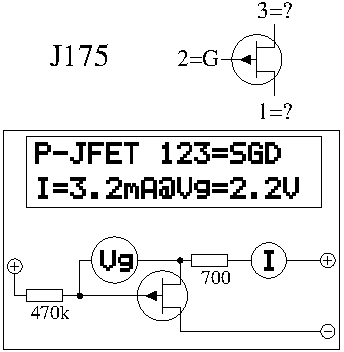
\includegraphics[width=1.\textwidth]{../FIG/JFET_J175.pdf}
    \caption{P-JFET}
    \label{fig:P-JFET}
  \end{subfigure}
  \caption{JFETs}
\end{figure}



